\documentclass[12pt,a4paper,titlepage]{article}
\usepackage{style}
\usepackage{pdfpages}
\usepackage{eso-pic}
\graphicspath{ {../figures/} }% figures are taken from this folder
% the document should be compiled with pdfLaTex

\begin{document}
\pagenumbering{gobble}

\phantomsection

%##############################################################################

% WikiBooks (http://en.wikibooks.org/wiki/LaTeX/Title_Creation)
%
% License:
% CC BY-NC-SA 3.0 (http://creativecommons.org/licenses/by-nc-sa/3.0/)
% 
% Instructions for using this template:
% This title page is capable of being compiled as is. This is not useful for 
% including it in another document. To do this, you have two options: 
%
% 1) Copy/paste everything between \begin{document} and \end{document} 
% starting at \begin{titlepage} and paste this into another LaTeX file where you 
% want your title page.
% OR
% 2) Remove everything outside the \begin{titlepage} and \end{titlepage} and 
% move this file to the same directory as the LaTeX file you wish to add it to. 
% Then add \input{./title_page_1.tex} to your LaTeX file where you want your
% title page.
%
%%%%%%%%%%%%%%%%%%%%%%%%%%%%%%%%%%%%%%%%%

%----------------------------------------------------------------------------------------
%	PACKAGES AND OTHER DOCUMENT CONFIGURATIONS
%----------------------------------------------------------------------------------------




\begin{titlepage}

\newcommand{\HRule}{\rule{\linewidth}{0.5mm}} % Defines a new command for the horizontal lines, change thickness here

\center % Center everything on the page
 
%----------------------------------------------------------------------------------------
%	HEADING SECTIONS
%----------------------------------------------------------------------------------------

Ministerul Educației al Republicii Moldova\\ % Name of your university/college
\textbf{Universitatea Tehnică a Moldovei}\\% Name of your university/college
Facultatea de Calculatoare, Informatica și Microelectronică\\
Filiera Anglofonă "Computer Science"\\


\vspace{2cm}



\hfill Admis la susținere\\
\hfill Prof. dr. hab. Viorel Bostan\\
\hfill Director Filieră Anglofonă\\

\vspace{0.4cm}
\hfill \rule{5cm}{0.2mm}\\
\hfill "\rule{0.75cm}{0.2mm}" \ \rule{3cm}{0.2mm} 2016
\vspace{3cm}




\begin{center}
{\LARGE \textbf{Utility Application for Hand Kinetotherapy}}\\
\vspace{0.6cm}
Proiect de licență
\end{center}
\vspace{1cm}


\hfill Student: \rule{3.9cm}{0.2mm}(N.Barbaroș)\\
\vspace{0.2cm}
\hfill Conducator: \rule{4cm}{0.2mm}(D.Ciorbă)\\
\vspace{0.2cm}
\hfill Consultanți: \rule{4.2cm}{0.2mm}(G.Covdii)\\
\vspace{0.2cm}
\hfill \rule{4cm}{0.2mm}(M.Balan)\\
\vspace{0.2cm}
\hfill \rule{3.9cm}{0.2mm}(E.Gogoi)\\
\vspace{0.2cm}
\hfill \rule{4cm}{0.2mm}(V.Bostan)\\
\vspace{4cm}



% If you don't want a supervisor, uncomment the two lines below and remove the section above
%\Large \emph{Author:}\\
%John \textsc{Smith}\\[3cm] % Your name

%----------------------------------------------------------------------------------------
%	DATE SECTION
%----------------------------------------------------------------------------------------
\begin{center}
Chișinău 2016
\end{center}
%{\large \today}\\[3cm] % Date, change the \today to a set date if you want to be precise

%----------------------------------------------------------------------------------------
%	LOGO SECTION
%----------------------------------------------------------------------------------------

%\includegraphics{Logo}\\[1cm] % Include a department/university logo - this will require the graphicx package
 
%----------------------------------------------------------------------------------------

\vfill % Fill the rest of the page with whitespace

\end{titlepage}


\cleardoublepage

\section*{Abstract}


The \textbf{Utility Application for Hand Kinetotherapy} presented by student Barbaroș Nicolae as a Bachelor project and it was developed at the Technical University of Moldova. It is written in English and contains 66 pages, 19 figures, 22 listings and 16 references. The thesis consist of a list of figures, list of abbreviations, list of listings,introduction, four chapters, conclusions, and references list.


The thesis has the object of studying the existing solution in the market of a rehabilitation system of an patient that got a stroke, hand fracture or a surgery and followed hand pain or hand paralysis and eventually creation of an application that  will aim to treat patients with hand pain, tendons injuries and neuro disorders.


With the help of Leap Motion technology, the application is capable to track the users hands in realtime. Using the tracked data offered by the controller about hand activities, the user is provided with a set of well defined exercises for a great rehabilitation experience and a feedback sistem so that every time the user will do an exercise, he will be notified about the correctness of the did exercise and the counted done exercises.

Hence the application does not require the use of extra complicated objects that will track users hand and only a small, easy, cheaper device that is connected only by an USB cable to the laptop, the user will be capable of having the device by his side and even in an airplain he can connect the device to the laptop, open the application, and start exercising.


The four chapter which compose the report are: the problem, domain analysis and the purposed
solution chapter. The second one is the used technologies and implementation chapter, followed by
the UML description of the system and user experience chapter, concluding with the chapter four
about the economical analysis of the system. The first chapter describes the problem that was identified and defines the solution. It also has a deep analysis of the market and existing solutions.
In the chapter two are presented the UML diagrams of the system and is listed the benefits of the user when using this application. In chapter three are presented the used technologies and some basic instructions on how to use
them. Also there is described the implementation part with sample listings of code. In the last
chapter is made a economical analysis in which are shown the total expenses, possible incomes and
is analysed the profitability of the project. This document is for readers with technical background,
engineers, IT students and programmers

\clearpage

\section*{Rezumat}

Teza \textbf{Modele matematice şi metode de eficientizare a conversiei energiilor regenerabile
 în baza efectelor aero-hidrodinamice}, prezentată de către Viorel Bostan pentru 
conferirea gradului ştiinţific de doctor habilitat în tehnică, a fost elaborată la Universitatea Tehnică a Moldovei, Chişinău, este scrisă în limba română şi conţine 342 pagini, 90 de figuri, 38 tabele, şi 250 de titluri bibliografice. Structura tezei include: introducerea, 6 capitole, concluzii şi anexe. Anexele conţin 145 de pagini cu 52 de figuri şi 48 tabele.
	
Teza este consacrată studiului fenomenelor aero-hidrodinamice în rotoarele turbinelor eoliene (TE) şi microhidrocentralelor de flux (MCHF) de mică putere ($P<20$ kW), cu aplicarea modelelor matematice de descriere a fizicii curgerii fluidelor şi a metodelor moderne de simulare numerică a turbulenţei din cadrul dinamicii fluidelor CFD.
	
Scopul lucrării constă în sporirea eficienţei conversiei şi a capacităţilor funcţionale ale turbinelor eoliene şi microhidrocentralelor de flux de mică putere.
	
Au fost identificate modelele şi metodele matematice moderne de descriere a curgerii turbulente a fluidului, specifică rotoarelor de mică putere, cu evidenţierea efectelor aero-hidrodinamice tranzitorii şi în vecinătatea palelor. A fost argumentate profilurile aero-hidrodinamice ale palelor eficiente din punct de vedere al randamentului conversiei energiei şi în baza lor au fost elaborate concepte originale de rotoare aero-hidrodinamice.
	
În baza modelelor CAD ale rotoarelor propuse: au fost efectuate simulări CFD complexe ale curgerii tranzitorii a fluidului prin rotoare şi în vecinătatea palelor, cu determinarea gradului de influenţă a parametrilor constructiv-cinematici asupra caracteristicilor de putere şi factorilor de performanţă aero-hidrodinamică a rotoarelor TE şi MHCF; a fost efectuată analiza fenomenului de curgere a fluidului în stratul limită şi identificate soluţii tehnice de control şi minimizare a impactului negativ al acestuia asupra eficienţei conversiei energiei.

În baza rezultatelor cercetărilor, au fost elaborate şi fabricate modele noi de TE şi MHCF pentru diverse aplicaţii, inclusiv conceptul TE cu rotor basculant şi orientare la direcţia curenţilor de aer cu windrose cu profil aerodinamic al palelor. Soluţiile tehnice elaborate au fost protejate cu 17 brevete de invenţie şi apreciate la saloanele internaţionale de inovaţii, cercetare şi transfer tehnologic cu 43 medalii de aur, 13 de argint şi 2 de bronz.

Cuvinte-cheie: modele matematice; simulare numerică CFD; strat limită; curgere turbulentă, rotor aero-hidrodinamic, turbină eoliană; microhidrocentrală.
\clearpage

\tableofcontents
\addtocontents{toc}{\protect\thispagestyle{empty}} 3.
\cleardoublepage

\pagenumbering{arabic}
\setcounter{page}{10}
\listoffigures
\addcontentsline{toc}{section}{List of figures}
\clearpage

\lstlistoflistings
\addcontentsline{toc}{section}{Listings}
\thispagestyle{empty}
\clearpage


\phantomsection
\addcontentsline{toc}{section}{Abbreviations}
\section*{Abbreviations}

\begin{itemize}[leftmargin=2cm, topsep=0pt, partopsep=5pt,itemsep=0pt,parsep=0pt]
\item [API] Application Programming Interface
\item [CIMT] Constraint Induced Movement Therapy
\item [IR] Infrared
\item[OM] Online Marketing
\item [NUI] Natural User Interface
\item [LED] Light-Emitting Diode
\item[SM] Social Media
\item [SaaS] Software as a Service
\item[UX] Experienta Utilizatorului
\item[UML] Unified Modeling Language
\item[UX] User Experience
\item[UI] User Interface
\item[VR] Virtual Reality
\end{itemize}
\thispagestyle{empty}
\cleardoublepage

\phantomsection
\addcontentsline{toc}{section}{Introduction}
\section*{Introduction}
%\phantomsection

Whether you are an athlete, or you had an undergone surgery, or maybe you are just an usuall human being hoping to rid yourself of hand pain -- kinetotherapy is a great recovery strategy to help get read or heal off your injury. The goal of kinetotherapy is getting read of injures as much as possible and promote muscular function and mobility, to work the muscles and the area with an injury, to strengthen the muscles and joints so that they perform better.
Instead of depending on drug usage kinetotherapy recommends to rely on the body's ordinary resources of physical recovery through exercises.

Due to the expansions of medical-related technology new types of rehabilitation of patients are introduces. Here comes Kyno, a desktop application that helps users through rehabilitation by restoring movement and function of the hand which is affected by injury, illness or disability.

One of Kynos solutions, aims to treat patients with hand pain, tendons injuries and neuro disorders. With the help of a tracking device Kyno can manipulate the data and send the learning acitivy in the "virtual" environment, letting to patient's an open dor to focus more and pay attention to the details of their movements which might bring them closer to recovery.

Kyno is bringing a new wave of innovation and hope for patients everywhere. Among lots of benefits, it brings to the patients more fun while stretching and recovering their physical capacities. In my system the program with the help of Leap Motion device projects the patients hand onto a virtual environment shown on a screen. Then the patient by choosing one set of exercises will start performing it, which is aimed to improve their physical issue. While tradition kinetotherapy in most cases forces to use weights or other tools, kyno omits the usage of them. 

More then that traditional old kinetotherapy is forced to work in strict physical places, while using Kyno the patiens will not only strengthen their muscles or recover their injuries, but also will improve their cognitive abilities due to exploring a brand new borned application. He will have to understand how the application works and then how he should act in it. For instance, choosing what exercise to take involves decision taking(which on to choose), motor skill (moving the mouse over a button and then click it), attention (sustaining concentration on the virtual hand while performing the exercise it is a brain challenge). 

The program uses infrared light with a wavelength of 850 nanometers, which is outside the visible light spectrum
to track and analyze the movement of objects that are withing the range of the Leap Motion controller that connects the real world with the computer. During therapy the patients stays in front of the screen with the hand above the controller, where he can watch his own hands generated in the virtual world among some UI. The patient's work is to choose one type of exercise provided by the application, to read the instructions and start the process of rehabilitation. Modern technology works in a fraction of a second, so thanks to that the application is able to provide a realtime feedback that indicates if the exercises were done correctly or not. The application is designed with 3 exercises that are intended to improve the motor skills and neuro capability of the hand and fingers.

This thesis is composed of 4 chapters, a list of abbreviations, a list of figures, a table of contents, conclusion and reference. The report has roughly 70 pages. Starting with the first chapter where its been described the problem that needs to be solved, the solution that is purposed and the current market analysis.The second chapter describes the system architecture via UML diagrams and has a succint description of the UX. The third chapter is mostly about the technologies that are used and describes how the system is realized, with chunks of sample code listings.  The fourth chapter analyses the project from the point of economics view, where the expenses of building the project, the marketing plan and the profit it can make can be seen. 
\cleardoublepage

\section{System analysis}
\phantomsection

\subsection{Motivation and the problem description}
A stroke\cite{whatisstroke} is a brain attack. It happens when the blood supply to part of your brain is cut off. Can be a devastating experience, leaving the patient with serious physical impairments and beset by concerns for the future. Today, that future is much brighter, as stroke rehabilitation has made enormous strides. 
First, and most importantly, researchers are working to improve patients’ compliance with their rehabilitation regimen, since up to 65 \% \cite{assesment} of patients fail to adhere fully—or at all—with their programs. In addition, they are addressing the lack of accessibility and the high cost associated with rehabilitation. If you have just had a stroke, even getting to the clinic is a challenge, and the cost of hiring a private physical therapist to come to your home is too high for most people.

\subsubsection{Physical challenges after stroke}

All strokes are different so for some people the effects may be relatively minor and may not last long, while others may be left with more serious long term problems.

A stroke can affect the way your body functions
Although all strokes are different, there are some common physical problems that many people experience:

\begin{itemize}
\item \textbf{problems with movement and balance}, many people experience muscle weakness or paralysis after a stroke, which can affect your mobility and balance. This usually happens on one side of your body and can also cause a lot of pain and discomfort;
\item Problems with your vision;
\item Problems with swallowing;
\item Excessive tiredness.
\end{itemize}

But there are other effects that can not been seen. Some of the ‘hidden’ effects of stroke include:

\begin{itemize}
\item \textbf{Problem with communication},  many people have difficulty with speech and language after their stroke. A common communication problems, which affects around one third of stroke survivors, is aphasia. People with aphasia find it difficult to speak and understand what other people are saying to them, as well as reading and writing;

\item \textbf{Problems with memory and thinking}, it is very common to find that their short-term memory and concentration is affected by stroke, but it can also affect other thinking processes as well, such as problem-solving, planning and finding your way around;

\item \textbf{Changes to your emotions}, a stroke has an emotional impact, which can lead to problems like depression and anxiety. It can also make it more difficult to control your emotions;

\item Changes to your behaviour.
\end{itemize}

Given the statistics from \mbox{figure} \ref{sequence_exercise}, it is important to note that more and more humans everyday die of stroke related diseases which is a cause of concern. More than in Republic of Moldova, in 2008 the number of patients that had a stroke started from 13 000 in 2014 the number got more then 5 times bigger with over 70 000 stroke patients \cite{strokereferince}.
\begin{figure}[!h]
\centering
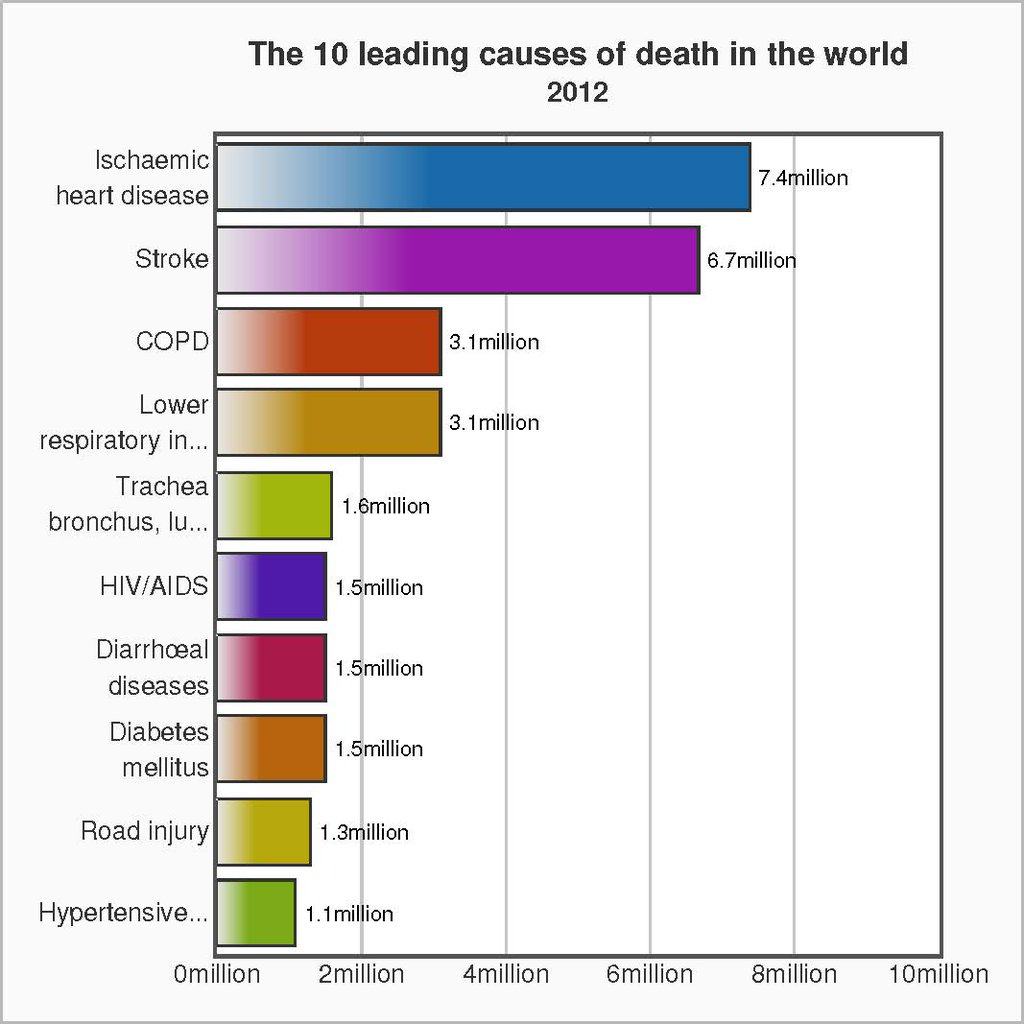
\includegraphics[width = 14cm]{stroke1}
\caption{Top 10 leading causes of death in the world 2012 \cite{strokeStatistic}}\label{stroke}
\end{figure}

\subsubsection{Physical therapy after stroke}

Movement problems affect each person differently.Different therapies may include:
\begin{itemize}
\item Practicing tasks/activities that you have difficulty doing. This may include rolling over in bed, sitting or standing up. It can also include walking and using your hand or arm;

\item Exercising to improve your strength, sensation (ability to sense or feel things), coordination, balance or fitness. Often this can be done as you practice normal activities such as standing or walking. Exercises that use electrical stimulation and other equipment (for example treadmills) may also be used as part of your therapy. This will help improve your ability to move;

\item Joining a fitness centre, club in the community, or exercise program at your local community health care centre. This can help to keep you fit. Often after a stroke, fitness levels drop. Therefore it is important to keep yourself as active as possible in the long-term. Talk to your therapist about how best to keep fit;

\item Learning how to walk safely. This may include the help of an aid like a frame or walking stick;

\item Limiting the use of your good arm to encourage use of the affected arm. This is called CIMT \cite{constrain}. Research has found that ‘forcing’ you to use your affected arm can improve recovery of your affected arm. It is important to talk to your therapist first.
\end{itemize}





\subsection{Stroke Case Study}
Now Consider Maria, a 56-year-old patient. After experiencing a stroke 5 months ago, she now has difficulty on controlling the left hand of her body. Like most stroke victims, Maria faces one to two weekly therapy sessions for up to 1 year. Unable to work, she worries about the fee per visit, as she has exhausted her insurance coverage. Maria also have to exercise hours daily to maintain her mobility. Unfortunately, the doctor gave her boring repetitive exercises, and Maria finds it diffucult to motivate herself to do them.

\textbf{What is the solution?}
Kyno offers a significant advance to help stroke patients restore their physical functions: an affordable motion-capture system for physical rehabilitation that uses Leap Motion technology.
Kyno tries to solves all of these issues by providing patients with "gamified" exercises that accelerate recovery and increase adherence. In addition, Kyno gives patients immediate feedback, which ensures that they perform their movements correctly. This is critical when the patient is exercising at home.



\subsection{Existing solutions and their drawbacks}
Before getting to implement the idea is better to do a market research for finding similar solutions to the problems that are being used by those applications.
\\
After analysing these solutions Kyno application will become better, stronger, different and adapted tool for local market and attractive for patient's and customers.
It is important to know what the user wants the most. What need to be done to make him happy, to make him have a great experience while using the software. Thats why more than that it is important to know the background for solution, the countless features that are counted as advantages and the ones that are not crucial. It is important to know what features will offer him confort or excitement. 

There was created a list of solutions after a quick research by searching the web for similar solutions and after to select only the best one, only those who have something common with Kyno, others where taken out, because the purpose of those application's wasn't as the purpose  of Kyno. The best existing solutions at the moment for patients kinetotherapy comes from big companies and these are: 

\begin{itemize}
\item VirtualRehab;
\item Jintronix;
\item SeeMe.
\end{itemize}

What I have seen, is that there are quite a lot of application of kinetoteraphy, each of them uses Microsoft Kinect to detect the motion, each of them is great amazing aplications but what is the problem in them is that each of them detects the full body of the patients and is provided most of the times with exercises/list of mini games where you have to move. However that is bad for patients that are paralyzed, that can't walk, that can't even move their legs.


\subsubsection{VirtualRehab application}
The first solution to kinetotherapy rehabilitation is \textit{www.virtualrehab.info}. In my opinion it is one of the most powerful rehabilitation application on the market. 

This tool provides functional training so as to improve equilibrium, coordination, weakness, fatigue and spasticity. The exercises can be adapted to a patient’s disability levels so that the programme can be used with a wide range of ability levels.

The strong advantage of VirtualRehab is that it has 2 type of application VirtualRehab Body and VirtualRehab Hands. 
VirtualRehab Body is a suite of therapeutic
games designed to help retrain upper and lower
limb motor functions.
Through the use of a variety of highly motivating
games, the system makes it possible to retrain
abilities such as balance (while sitting and
standing), thrust inhibition, load transfer
and changing between sitting and standing
positions. VirtualRehab Hands works the mobility and
strengthening of the muscles used in flexion,
joining, separation and extension of the fingers. This possibility offers to cover a full controll of body rehabilitation.

A second great advantage is that the rehabilitation process in VirtualRehab is made through games. It has 9 games that help treat various physical symptoms.

Another great feature is the feedback system of this applications. With the help of Kinect they are capable to keep track of progress and give feedback in real time to the patient about the correct or incorrect movement performes. This feature is going to be implemented in Kyno.

Even more it has a simple patient management panel. It ncludes an easy to use therapy editor that allows therapists to program customized therapy sessions taking into account each patient’s particular needs.  All the information from the sessions is stored in the data server immediately making it possible to track and monitor each patient´s progress in the prescribed therapy.
\subsubsection{Jintronix application}
Jintronix is transforming rehabilitation by providing an innovative, accessible and value-driven model for the delivery of physical and occupational therapy. 

Combining kinect motion tracking, virtual gaming and remote clinical monitoring, Jintronix offers patients a fun and effective tool for their rehabilitation through games. 
The games were developed through researching which exercises and sports best fitted with conventional therapy. The rehab modules are adaptable to the level of a patient's functional and cognitive abilities and are designed to train balance and mobility, muscle strengthening and endurance, flexibility and range of motion, fall prevention, postural control, motor control and relearning and bilateral coordination. Jintronix is capable of tracking a players’ movements to see whether they are performing the activities correctly and relays this to the therapist who can then make adjustments. So far, there are seven games that have been created and work smoothly.

\subsubsection{SeeMe application}
A third solution to Kyno is  SeeMe at \textit{www.virtual-reality-rehabilitation.info}
SeeMe provides active training in the form of games – what
makes patients more motivated to participate in their
rehabilitation process. SeeMe creates a feedback loop
between a patient performing rehabilitation exercises and
a physical therapist. In real time the physical therapist can
monitor the patient’s performance and adjust
parameters of current “gamified” exercise to match the
patient’s individual recovery needs.

These are the great key features of SeeMe at this moment:
\begin{itemize}
\item \textbf{ Deep Customization}, each exercise can be personally customized to meed the specific requirements of the patient. All the tasks customizations can be done in real time while patient is playing;

\item \textbf{Many Applicaitons}, SeeMe uses a wide variety of therapeutic tasks to enable training in all rehabilitation domains;

\item \textbf{Engaging Activities}, all the therapeutic tasks included in SeeMe offer plety of paratemters and leverls. By having those options - therapists are able to prepare trainings that let patients experience positive emotions, keep motivation, become more self-confident and in the same time remain challenged;

\item \textbf{Powerful Reports}, enables detailed insight into the course of each training and long-term progress as well. Therapists can collect objective results of treatment progress.


\end{itemize}

SeeMe it is a very comprehnsive tool which makes the patient/user happy, it brings to the patient a new way of rehabilitation, home rehabilitation with lots of interactive fun to play games.


\subsection {Proposed solution}

Kyno tries to solves all of these issues by providing patients with "gamified" exercises that accelerate recovery and increase adherence. In addition, Kyno gives patients immediate feedback, which ensures that they perform their movements correctly. This is critical when the patient is exercising at home. However to create a really useful application, it is important to know what the market really needs.

Kyno should be capable of giving the following solutions :

\begin{itemize}
\item Helping getting read of injuries, promote muscular function and mobility, to work muscles and the area with injuries, strengthen the muscles and joints so that they perform better;
\item During the exercise the tools that will help on rehabilitation will be the users hands only(not other tools, weights);

\item The UI should be intuitive, easy to use, clean and not very complicated. The UX must be great with not so many pop ups, additional panels. The application should provide to the user at least 3 options of exercises which are most used and most useful for injuries recovery;
\item Have a price accordingly to the local and external market. Current solutions that involves technologies are way way more expensive then what it is proprosed. Thus, the price range must be affordable for the local and external market;
\item The application will be developed and build for desktop's with later support for Virtual Reality which will give a brand new exited experience for patients.
\end{itemize}

There are numerous rehabilitation hand exercises to which Kyno could work, but there should be chosed a couple of them for initial market test they are written in the itemized list further and for launching the project, after which there can be added other exercises as well. Also due to the Leap Motion device tracking limitation some of the exercises can not be included because Leap Motion is not able to "see through the fingers" - for example, when one finger covers the other. Fingers right next to each other also pose a problem for the cameras and might not be recognized individually. This is not a device which incorporates science fiction hardware with x-ray vision and magical recognition properties - even though some buyers on the bleeding edge might have expected exactly that. That's why some exercises cannot be done.
\begin{itemize}
\item \textbf{Grab}.
\item \textbf{Pinch}.
\item \textbf {Roll}.
\end{itemize}
Some key features/benefits of the application:
\begin{itemize}
\item \textbf{Gains}.Kyno will use a wide range of kinetotherapeutic exercises to train the following rehabilitation domains:

\textbf{Musculo-skeletal}
\begin{enumerate}
\item Range of motion;
\item Strength;
\item Endurance;
\item Fitness and cardiovascular training.
\end{enumerate}


\textbf{Balance and Equilibrum}
\begin{enumerate}
\item Self control;
\item Anticipatory postural responses;
\item Adequate reactions to stimuli and distractors placed in preplanned positions or random.
\end{enumerate}


\textbf{Neurological}
\begin{enumerate}
\item Hand movement quality;
\item Hand movement awareness and proprioception;
\item Bilateral movements in response to bilateral stimuli.
\end{enumerate}

\textbf{Cognition}
\begin{enumerate}
\item Memory;
\item Perception;
\item Planning and executive functions.
\end{enumerate}

\item \textbf{Engaging activities}. There is no
need to wear, hold or be attached to any
equipment – patients can almost forget it is
still a real rehabilitation.
\end{itemize}




\clearpage
\cleardoublepage

\section{ Implementation and Used Technologies}
\phantomsection

\clearpage
\cleardoublepage

\section{Architecture of the System}
\phantomsection

\clearpage
\cleardoublepage

\section{Economic Analysis}\label{sec:economy}
\phantomsection

\subsection{Project description}


Kyno project is a treatment application for patients who have suffered from physical injury or illness on hands. This application will be used to improve a person's endurance, mobility and strength in hand. The rehabilitation techniques used by kinetoteraphies are often prescribed to help individuals enhance their overall physical conditioning. A patient may see a kinetotherapist after receiving a prescription from a physician, physician assistant or nurse practitioner. Kinetotherapists primarily work in public and private hospitals, sports medicine facilities, rehabilitation centers and academic institutions, as well as in private practice and as consultants. Which puts them as my main marketing targets.  The success of this application will dramatically increase if we cross the countries borders, since there private hospitals, sports medicine have more money to invest and are willing to have better system of pacient treatment.

There are multiple solutions which provide kinetoteraphy application, but there is no other
similar product in Moldova. The main advantage is that it’s simple to use, it has a nice UX and UI, it gives feedback in a pleasant way and it has a system that tells you if the exercise was done well. It's perfect for everybody as soon as it has the required tools. That’s why it is expected to be a promising product, with other possibilities which are going to be implemented in future.


\subsection{SWOT analysis}
It is necessary to make an analysis of strong and weak points for the given application, in order to have a
brief overview about expectations or about possible problems that can appear. In \ref{table:swot} it is represented
the strategic planning method, called SWOT, used to evaluate Strength, Weaknesses, Opportunities and
Threads involved in the project.


\begin{table}[!ht]
\begin{center}
\caption{SWOT analysis}
\renewcommand{\arraystretch}{2}


\begin{tabular}{|>{\centering\arraybackslash}p{8cm}|>{\centering\arraybackslash}p{8cm}|}
\hline
\textbf{Strengths} & \textbf{Weaknesses}\\
\hline
\parbox{7.9cm}{\begin{itemize}
                     \item it is a new product on the market
                     \item easy to use
                     \item price, value, quality
                     
                  \end{itemize} }&
\parbox{7.9cm}{\begin{itemize}
                     \item You need LeapMotion devise in order to use it
                     \item client application available only on Windows platform
                     \item lack of funding
                     \item location and geography

                  \end{itemize} }\\
\hline
\textbf{Opportunities} & \textbf{Threads}\\
\hline
\parbox{7.9cm}{\begin{itemize}
                     \item it save time and money to the client
                     \item extendable to more regions
                     \item outsourced labor for development
                     \item not yet mature
                     \item time to market

                  \end{itemize} }&
\parbox{7.9cm}{\begin{itemize}
                     \item won't be bought by hospitals
                     \item similar application can be developed, so the popularity of this system may decrease
                     \item integration with existing systems
                     \item technical challenges
                  \end{itemize} }\\
\hline
\end{tabular} 

\label{table:swot}
\vspace{-2.5em}
\end{center}
\end{table}
\newpage
After elaboration of SWOT Analysis, it was taken in consideration the objective of the business
venture of project and there were identified the internal and external factors that are favorable and
unfavorable to achieve the goal. There will always be concurrency, this factor having an important role in
market development and increase of systems’ quality.



\subsection{Project time schedule}
For the accomplishment of a project it is necessary to establish a schedule. For the development of the Kyno application, agile project management is applied to offer flexible and iterative method of designing the application. It goes in 5 stages: planning, research, development, testing and deployment. The process flows in repetitive and incremental way.


\subsubsection{Objective determination}
The main objective of the following project is to provide a complete and functioning application for it's users. Otherwise without a finished product there is no profit. More to that, it is important to market the application and get exposed to a large audience in need. This can be done by targeting first private hospitals. Since it is not a common piece of software, it creates a very specific audience of users.

To keep up with the latest trends and researches, it is also an essential objective to keep updated and provide enhancements to the software. The lifecycle of the application will require bugfixes, interface changes, feature implementations. All of that will help the system still be trendy and up-to-date on the market.
\subsubsection{Time schedule establishment}
As it was said above the project will iterate over 5 steps: planning, research, development, testing and deployment. Naturally as most of the IT projects, it is subdivided into smaller parts. Planning step isn't supposed take up a lot of time, since the requirements are flexible. Moreover due to the research part the design solutions can change over time and open up new perspectives. The process of development is being split up in smaller tasks that can be accomplished within a 2-5 day period. Total duration of the project is computed using \eqref{eq:duration}.

\begin{equation} \label{eq:duration}
 D_T = D_F - D_S + T_R,
\end{equation}

\noindent
where $D_T$ is the duration, $D_F$ -- the finish date, $D_S$ -- the start date and $T_R$ -- reserve time. In table \ref{table:schedule} is presented the first iteration of the project schedule. It uses the following notations: PM -- project manager, SM -- sales manager, D -- developer/designer, T -- Tester.

\begin{table}[!ht]
\begin{center}
\caption{Time schedule}
\renewcommand{\arraystretch}{2}
\begin{tabular}{| c | >{\centering\arraybackslash}p{5cm} | >{\centering\arraybackslash}p{2cm} | c | >{\centering\arraybackslash}p{5cm} |}
\hline
\textbf{Nr} & \textbf{Activity Name} & \textbf{Duration (days)} & \textbf{People involved} & \textbf{Notes} \\
\hline
1 & Define the project concept and objectives & 10 & PM, SM, D &  \\
\hline
2 & Perform market analysis & 10 & PM, SM & Market analasys document \\
\hline
3 & Analysis of the domain & 10 & D & Research of algorithms and technologies \\
\hline
4 & Requirements and specifications & 5 & PM, D & Write them down \\
\hline
5 & System design & 10 & PM, D & UML  \\
\hline
6 & Preprocessing and learning part of the implementation & 25 & PM, D & \\
\hline
7 & End-user application development & 30 & PM, T, D, SM & This includes UX and UI design \\
\hline
8 & Validation of results & 5 & PM, T, D, SM & \\
\hline
9 & Documentation & 5 & D & \\
\hline
10 & Building and testing the entire project & 15 & PM, T, D & Real users for testing\\
\hline
11 & Active marketing & 15 & SM & OM on SM and private hospitals\\ 
\hline
12 & Total time & 140 & & \\
\hline
\end{tabular}
\label{table:schedule}
\vspace{-2.5em}
\end{center}
\end{table}
\newpage
Table \ref{table:schedule} shows the activities that will occur during project development, who is involved into each process and how much time does it take to accomplish a task. Total amount of time spent on this project is 140 days or 20 weeks, which means almost 5 months for a strong beta version.
For each individual, it is indicated below the number
of spent days:
 \begin{itemize}
 \item PM: 110 days;
 \item SM: 70 days;
 \item D: 115 days;
 \item T: 50 days
\end{itemize}

\subsection{Economic motivation}
The following section describes the evaluation of the project from the economic point of view. That includes the total profit, number of potential clients, salaries that have to be paid to employees, revenues that the company gets by commercializing the product. All the costs and prices are given in MDL (Moldavian lei) currency. Tangible and intangible assets, indirect expenses will also be taken into account. Wear and depression in regard to final product will also be computed.The entire economical part is done on the presumption that the software will have payed licenses. Either way it is a curios approach to compute all the necessary resources and indexes for developing a project. It opens managerial insights over entrepreneurial ideas.


\subsubsection{Tangible and intangible asset expenses}
The budget for the required tangible and intangible assets is shown in Table \ref{table:tangible_assets}, Table \ref{table:intangible_assets}. Direct expenses are presented in Table \ref{table:direct_expenses}.

\begin{table}[!hb]
\begin{center}
\caption{Tangible asset expenses}
\renewcommand{\arraystretch}{2}
\begin{tabular}{| c | c | >{\centering\arraybackslash}p{2.7cm} | >{\centering\arraybackslash}p{2cm} | c | >{\centering\arraybackslash}p{5em}|}
\hline
\textbf{Material} & \textbf{Specification} & \textbf{Measurement unit} & \textbf{Price per unit (MDL)} & \textbf{Quantity} & \textbf{Sum (MDL)}\\
\hline
Mac Book pro & retina display i7 & Unit & 25000 & 2 &  \multicolumn{1}{r|}{50000}\\
\hline
Apple Display & 27 inch & Unit & 20000 & 2 &  \multicolumn{1}{r|}{20000}\\
\hline
Asus laptop & K55VD, i5 & Unit & 5000 & 1 & \multicolumn{1}{r|}{5000}\\
\hline
Leap Motion & hand controller 5 & Unit & 1600 & 2 & \multicolumn{1}{r|}{3200}\\
\hline
\multicolumn{5}{|r|}{Total} & \multicolumn{1}{r|}{78200}\\
\hline
\end{tabular}
\label{table:tangible_assets}
\end{center}
\vspace{-1.3em}
\end{table}

\newpage
\begin{table}[!hb]
\begin{center}
\caption{Intangible asset expenses}
\renewcommand{\arraystretch}{2}
\begin{tabular}{| c | c | >{\centering\arraybackslash}p{2.7cm} | >{\centering\arraybackslash}p{2cm} | c | >{\centering\arraybackslash}p{5em}|}
\hline
\textbf{Material} & \textbf{Specification} & \textbf{Measurement unit} & \textbf{Price per unit (MDL)} & \textbf{Quantity} & \textbf{Sum (MDL)} \\
\hline

Unity Pro & Subscription &Unit & 1500 & 1 & \multicolumn{1}{r|}{1500} \\
\hline
VS Professional 2015& License & Unit & 10000 & 1 & \multicolumn{1}{r|}{10000}\\ 
\hline
Enterprise Architect &Home& Unit & 1900 & 1 & \multicolumn{1}{r|}{1900}\\ 
\hline
Windows 10 &License& Unit & 2400 & 1 & \multicolumn{1}{r|}{2400}\\ 
\hline
MS Word 2016 &License& Unit &1400& 1 & \multicolumn{1}{r|}{1400}\\ 
\hline
Adobe Illustrator &Subscription& Unit &1000& 1 & \multicolumn{1}{r|}{1000}\\ 
\hline
\multicolumn{5}{|r|}{Total} & \multicolumn{1}{r|}{18200}\\
\hline
\end{tabular}
\label{table:intangible_assets}
\vspace{-1em}
\end{center}
\end{table}


\begin{table}[!hb]
\begin{center}
\caption{Direct expenses}
\renewcommand{\arraystretch}{2}
\begin{tabular}{| >{\centering\arraybackslash}p{5em} | >{\centering\arraybackslash}p{7em} | >{\centering\arraybackslash}p{7em} | >{\centering\arraybackslash}p{5em} | >{\centering\arraybackslash}p{5em} | r |}
\hline
\textbf{Material} & \textbf{Specification} & \textbf{Measurement unit} & \textbf{Price per unit (MDL)} & \textbf{Quantity} & \multicolumn{1}{>{\centering\arraybackslash}p{5em}|}{\textbf{Sum (MDL)}}\\
\hline
Whiteboard & Universal Dry Erase Board & Unit & 400 & 1 & 400 \\
\hline
Post-it note & Stickers & Unit & 20 & 10 & 200 \\
\hline
Paper & A4 & 500 sheets & 60 & 1 & 60 \\
\hline
Marker & Whiteboard marker & Unit & 15 & 10 & 150 \\
\hline
Pen & Blue pen & Unit & 5 & 20 & 100 \\
\hline
\multicolumn{5}{|r|}{Total} & 910 \\
\hline
\end{tabular}
\label{table:direct_expenses}
\vspace{-1.5em}
\end{center}
\end{table}


The total amount of expenses in MDL is about this much.

\begin{equation}
 T_{e} = 78200 + 18200 = 96400
\end{equation}

\subsubsection{Salary expenses}
This section is concerned about the salaries to employees and various funds that should be paid. The distribution of salaries per day is the following: project manager - 500MDL, tester - 350 MDL, sales manager - 400 MDL, developer - 480 MDL.

\begin{table}[!ht]
\begin{center}
\caption{Salary expenses}
\renewcommand{\arraystretch}{2}
\begin{tabular}{| >{\centering\arraybackslash}p{8em} | >{\centering\arraybackslash}p{8em} | >{\centering\arraybackslash}p{8em} | r |}
\hline
\textbf{Employee} & \textbf{Work fund (days)} & \textbf{Salary per day (MDL)} & \multicolumn{1}{>{\centering\arraybackslash}p{5em}|}{\textbf{Salary fund (MDL)}}\\
\hline
Project Manager & 110 & 500 & 55000 \\
\hline 
Tester & 50 & 350 & 17500\\
\hline
Sales Manager & 70 & 400 & 28000\\
\hline
Developer & 115 & 480 & 55200\\
\hline
\multicolumn{3}{|r|}{Total} & 155700\\
\hline
\end{tabular}
\label{table:salaries}
\vspace{-2.5em}
\end{center}
\end{table}

Now by having computed all the salaries for the employees, it is time to compute how much to be paid to social services fund, medical insurance fund and the total work expenses by summing up all previous expenses. 

Salary expenses are introduces in Table \ref{table:salaries}.

This year the social service fund is approved to be $23\%$, therefore the salary expenses are computed according to the relation \eqref{eq:fs}.

\begin{equation}\label{eq:fs}
\begin{split}
 FS &= F_{re} \cdot T_{fs} \\
    &= 155700 \cdot 23 \% \\
    &= 35811
\end{split}
\end{equation}
\noindent
where $FS$ is the salary expense, $F_{re}$ is the salary expense fund and $T_{fs}$ is the social service tax approved each year. The medical insurance fund is computed as

\begin{equation}
\begin{split}
 MI &= F_{re} \cdot T_{mi}\\ 
    &= 155700 \cdot 4.5\%\\ 
    &= 7006.5
 \end{split}
\end{equation}

\noindent
where $T_{mi}$ is the mandatory medical insurance tax approved each year by law of medical insurance and this year it is $4.5\%$. 

So now having computed social service tax and medical insurance tax, it is possible to compute total work expense fund as follows

\begin{equation}
\begin{split}
 WEF &= F_{re} + FS + MI\\
     &= 155700 + 35811 + 7007\\
     &= 198.518
\end{split}
\end{equation}

\noindent
where $WEF$ is the work expense fund, FS is the social fund and MI is the medical insurance fund. In that way the total work expense fund was computed.


\subsection{Individual person salary}
Along with total work expense fund, it is necessary to compute the annual salary for the project manager. Considering that the project manager has a salary of 500 MDL per day and there are approximately 256 working days in the year, so the gross salary that the project manager get is

\begin{equation}
 GS = 400 \cdot 256 = 102400
\end{equation}

\noindent where $GS$ is the gross salary computed in MDL.

Social fund tax this year represents $6\%$, so the amount that should be tax paid in MDL represents

\begin{equation}
 SF = 102400 \cdot 6\% = 6144
\end{equation}

Medical insurance tax represents $4.5\%$ and gives the following result

\begin{equation}
 MIF = 102400 \cdot 4.5\% = 4608
\end{equation}

In order to proceed with income tax computations, it is necessary to calculate the amount of taxed salary.

\begin{equation}
\begin{split}
 TS &= GS - SF - MIF - PE \\
              &= 102400 - 6144 - 4608 - 10128\\ 
              &= 81520
\end{split}
\end{equation}

\noindent
where $TS$ is the taxed salary, $GS$ -- gross salary, $SF$ -- social fund, $PE$ -- personal exemption, which this year is approved to be $10128$.

The last but not the least thing to be computed is the total income tax, which is $7\%$ for income under 29640 MDL and $18\%$ for income over 29640 MDL.

\begin{equation}
\begin{split}
 IT &= TS - ST \\
      &= 29640 \cdot 7\% + 51880 \cdot 18\% \\
      & = 2074.8 + 9338.4 = 11413.2
 \end{split}
\end{equation}

\noindent
where $IT$ is the income tax, $TS$ -- the taxed salary and $ST$ -- the salary tax. With all this now it is possible to find out what's going to be the net income.

\begin{equation}
\begin{split}
 NS &= GS - IT - SF - MIF \\
            &= 102400 - 11413.2 - 6144 - 4608 \\
            &= 80.234.8
\end{split}
\end{equation}

\noindent
where $NS$ is the net salary, $GS$ -- gross salary, $IT$ -- income tax, $SF$ -- social fund, $MIF$ -- medical insurance fund.

\subsubsection{Indirect expenses}
The indirect expenses are things like electricity, Internet traffic, water, etc. Those will be presented in Table \ref{table:indirect_expenses}.

\begin{table}[!ht]
\begin{center}
\caption{Indirect expenses}
\renewcommand{\arraystretch}{2}
\begin{tabular}{| >{\centering\arraybackslash}p{5em} | >{\centering\arraybackslash}p{7em} | >{\centering\arraybackslash}p{7em} | >{\centering\arraybackslash}p{5em} | >{\centering\arraybackslash}p{5em} | r |}
\hline
\textbf{Material} & \textbf{Specification} & \textbf{Measurement unit} & \textbf{Price per unit (MDL)} & \textbf{Quantity} & \multicolumn{1}{>{\centering\arraybackslash}p{4em}|}{\textbf{Sum (MDL)}}\\
\hline
Internet & Moldtelecom & Pack & 200.00 & 1 & 200 \\
\hline
Transport & Public bus & Trip & 3.00 & 150 & 450\\
\hline
Office Leasing & Office & $m^2$ & 115 & 25 & 2875\\
\hline
Electricity & Union Fenosa & KWh & 2.16 & 1160 & 2505.6\\
\hline

\multicolumn{5}{|r|}{Total} & 6030.6 \\
\hline
\end{tabular}
\label{table:indirect_expenses}
\vspace{-2.5em}
\end{center}
\end{table}

\subsubsection{Wear and depreciation}
Another important part of economic analysis is the computation of wear and depreciation. It is a well known fact that any product decreases its value with time. Depression will be computed uniformly for the whole project duration, so that there are no accountancy issues. In other words, if a product is planned for 3 years, it should be divided into 3 uniform parts according to each year. 

Straight line depreciation will be applied. Normally wear is computed regarding to the type of asset. The notebook and single-board computer are usable for a period of 3 years. Licenses will last for a single year. At first tangible and intangible assets are summed up and then the salvage costs of each of the items at the end of their period of use has to be subtracted:

\begin{equation}
 \begin{split}
  TAV &= \sum_{} n(AC - SV) \\
        &= 2*(25000 - 1000)  + 2*(20000 - 1000) + (5000 - 1000) + 2*(1600 - 1000)\\&  + (1500 - 1000)+ (10000 - 1000) + (1900 - 1000) + (2400 - 1000)\\& + (1400 - 1000) + (1000 - 1000) \\
        &= 102400
 \end{split}
\end{equation}

\noindent
where $TAV$ is the total assets value, $AC$ -- assets cost, $SV$ -- salvage value, $n$ -- number of items. In order to get the yearly wear, divide total asset value by the period of use of assets, being 3 years.

\begin{equation} \label{eq:wear}
 \begin{split}
  W_y &= TAV / T_{use} \\
                &= 102400/3\\
                &= 34133
 \end{split}
\end{equation}

\noindent
where $W_y$ is the wear per year, $TAV$ -- total assets value, $T_{use}$ -- period of use. Relation \eqref{eq:wear} included tangible assets which will last for 3 years and intangible assets which last only one year. The initial value of assets in MDL was

\begin{equation}
 \begin{split}
  W &= W_y / D_y \cdot T_p\\
                   &= 34133  / 365  \cdot 140 \\
                   &= 13092
 \end{split}
\end{equation}

\subsubsection{Product cost}
With all the project expenses computed, it is easy to compute the product cost which includes the cost used to create this product. \ref{table:product_cost}.

\begin{table}[!ht]
\begin{center}
\caption{Total Product Cost}
\renewcommand{\arraystretch}{2}
\begin{tabular}{| >{\centering\arraybackslash}p{10em} | r | r |}
\hline
\textbf{Expense type} & \multicolumn{1}{>{\centering\arraybackslash}p{6em}|}{\textbf{Sum (MDL)}} & \multicolumn{1}{>{\centering\arraybackslash}p{6em}|}{\textbf{Percentage (\%)}}\\
\hline
Direct expenses & 18200 & 9.67 \\
\hline
Indirect expenses & 910 & 0.49 \\
\hline
Salary expenses & 155700 & 82.87\\
\hline
Asset wear expenses & 13092 & 6.97 \\
\hline
\textbf{Total product cost} & \textbf{187902} & \textbf{100}\\
\hline
\end{tabular}
\label{table:product_cost}
\vspace{-2.5em}
\end{center}
\end{table}


\subsubsection{Economic indicators and results}
At this point it is crucial to sell the product to clients from mediacal sphere. The total product cost is very high, consequently there are 2 strategies that can be applied -- whether sell less with a high price or sell more with a lower price. It is not possible to add a percentage to the product cost that will represent the profit. It is assumed that the expected profit represents $20\%$ of the total product cost and the expected number of sold copies to be 300.

\begin{equation}
 \begin{split}
  GP &= C_{total} / N_{cs} + P_{p}\\
              &= 187902/400 + 20\% \\
              &= 563
 \end{split}
\end{equation}

\noindent
where $GP$ is the gross price, $C_{total}$ -- total product cost, $N_{cs}$ -- number of copies sold, $P_{p}$ -- chosen profit percentage. This is not the price of the end product, since it is necessary to add sales tax (VAT), which represents $20\%$ and is added to the gross price. 

\begin{equation}
 \begin{split}
  P_{sale} &= GP + TX_{sales}\\
              &= 563 + 20\% \\
              &= 675.6
 \end{split}
\end{equation}

\noindent
where $P_{sale}$ is the sale prices including VAT, $GP$ -- gross price, $TX_{sales}$ -- sales tax. The net income is computed by multiplying gross price and the number of expected copies to be sold, which will be

\begin{equation}
 \begin{split}
  I_{net} &= GP \cdot N_{cs}\\
              &= 675.6  \cdot 300 \\
              &= 202680
 \end{split}
\end{equation}

\noindent
where $I_{net}$ is the net income, $GP$ -- gross price, $N_{cs}$ -- number of copies sold. Moreover it is necessary to compute the gross and net profit. The indicators are $GPr$ -- gross profit and $NPr$ -- net profit.

\begin{equation}
 \begin{split}
  GPr &= I_{net} - C_{production}\\
              &= 202680 - 187902\\
              &= 14778\\
  NPr &= GPr - 12\% \\
             &= 14778 - 12\% \\
             &= 13004
 \end{split}
\end{equation}

\noindent
where $I_{net}$ is the net income, $C_{production}$ -- cost of production. The profitability indicators are $C_{profit}$ -- cost profitability, $S_{profit}$ -- sales profitability computed in MDL.

\begin{equation}
 \begin{split}
  C_{profit} &= GPr / C_{production} \cdot 100\%\\
              &= 14778 / 187902 \cdot 100\% \\
              &= 7.87 \%\\
  S_{profit} &= GPr / I_{net} \cdot 100\% \\
             &= 14778 / 202680 \cdot 100\% \\
             &= 7.30 \%
 \end{split}
\end{equation}

\subsection{Marketing Plan}
Concept of Marketing derived from the word market. Marketing - economical activities that guide flow of goods and services from producer to consumer.  Marketing is a system of economical activities about price setting, promotion and distribution of products and services to satisfy current and potential consumers requests. Marketing is the science and art of exploring, creating, and delivering value to satisfy the needs of a target market at a profit.

 Functions of Marketing:
 \begin{itemize}
 \item Analyzing of external environment;
 \item Analyzing consumers behavior;
 \item Development of product;
 \item Development of distribution;
 \item Development of promotion;
 \item Price setting;
 \item Social responsibility;
 \item Management marketing.
\end{itemize}

This application will be spread between private/public hospitals and people at home. To make people use a new application is not so easy because it needs time and investment to make it popular and well known.However the application will be easy to use so that an ordinary application user will be able to intuitively use it.

Market research stages:
\begin{itemize}
 \item Identifying the problem;
 \item Developing program of research and gathering;
information
 \item Establishing specific information ( internal, external );
 \item Establishing methods for collecting data;
 \item Performance of research;
 \item Information analysis, drawing conclusions.
\end{itemize}

Introduction stage This stage of the cycle could be the most expensive for a company launching a new product. The size of the market for the product is small, although they will be increasing. On the other hand, the cost of things like research and development, consumer testing, and the marketing needed to launch the product can be very high, especially if it's a competitive sector.

Strategy - Screaming, massive penetration The growth stage is typically characterized by a strong growth in sales and profits, and because the company can start to benefit from economies of scale in production, the profit margins, as well as the overall amount of profit, will increase. This makes it possible for businesses to invest more money in the promotional activity to maximize the potential of this growth stage.

Maturity Stage - During the maturity stage, the product is established and the aim for the manufacturer is now to maintain the market share they have built up. This is probably the most competitive time for most products and businesses need to invest wisely in any marketing they undertake. They also need to consider any product modifications or improvements to the production process which might give them a competitive advantage.

Declining stage - the market for a product will start to shrink, and this is what's known as the decline stage. This shrinkage could be due to the market becoming saturated (i.e. all the customers who will buy the product have already purchased it), or because the consumers are switching to a different type of product or even a new/better product.


\subsection{Economic conclusions}
Kyno project was analyzed from the economic point of view. It was computed the production cost, different profit and profitability indicators, various types of expenses involved, including direct, indirect, salary and taxes. The whole analysis is worth to understand if the product will be successful and if it's worth investing money in it. The biggest expense represents the intellectual equity, since it is critical to have a reliable product, which is based on extensive research and professional development techniques. The price of the application can become a blocker, therefore it's price might be dropped. In such scenario other means of profit can exist.

The commercialization of the product is not an easy task. High-quality service and customer support can be provided only to institutions and users that bought the product. The success of the product highly depends on financial strategy and solid economic analysis, which was presented in this chapter.
\cleardoublepage

\phantomsection
\addcontentsline{toc}{section}{Conclusions}
\section*{Conclusions}
\phantomsection

Kyno project is the result of the thesis work. It is an application that gives to the user exercises for kinetotherapy rehabilitation. The uniqueness of the application is that the targeted users and the proposed solution is unusual for the moldavian market. There are still no tools available that does a similar thing on the local level. However, developing a software that doesn't yet exist on a market offers a lot of freedom, but at the same time is problematic because the needs of the potential customers are yet blurry. A joint work with a the Physiotherapist representative would have resulted into a more specific and useful product.

There are other rehab systems out there that use motion capture, but they often require sensor gloves or other proprietary hardware that take a lot of training and supervision to use, or they depend on rigging an entire room with expensive cameras or placing lots of sensors on the body. Thanks to Leap Motion, Kyno doesn’t require any extra hardware, cameras, or body sensors, which keeps the price affordable,. That low price point is extremely important.

Kyno is working to remove all the major barriers to physical rehabilitation by making a system that is fun, simple to use, and affordable. Kyno demonstrates the potential of NUI to make technology simpler and more effective—and the ability of Leap Motion technology to help high tech meet essential human needs.

Building the application required many multi-step planning of the infrastructure. The first problem encountered with choosing what gestures to be detected in the app. Due to the Leap Motion device tracking limitation some of the exercises can not be included because Leap Motion is not able to "see through the fingers" - for example, when one finger covers the other. Fingers right next to each other also pose a problem for the cameras and might not be recognized individually. That's why some exercises cannot be done.


During first stage of marketing it is really important to collect feedback about the application from the clients and then releasing new versions with the implemented feedback. Also if the marketing want's to cross the border and wants to grow on international levels, the more functionalities should be implemented in the sistem.

One of the functionality to be implemented is a system that is  monitoring the progress of patients from anywhere in the world. Patients can perform complex rehabilitation programs using entertaining therapies either in a Rehabilitation clinic as well as in their own homes.

Each session will be registered using Microsoft® Azure, a cloud-based platform that will allow patients to complete therapy sessions under the supervision of their specialist, whether at a medical centre or at home.

An important part for the future development of Kyno is to add mini artificial inteligent component that will take the user through an amazing experience on how to use the application, how to put the hands over Leap Motion controller, how to perform certain exercises. So basically the component will tell the user to press one button so the user will have to do that, then it will say to the user to put his hands over Leap Motion and again user will have to act as the component shows. It will be runned every time the application was launched for the first time on a system after that it will just ask the user if he want to go through a tutorial.

Another future implementation is adding more exercises, which means detecting more gestures, then gamify them to create a better user experience. Gamified content makes users to establish a special excited relation between them and the application.


As a generalization, working on this project was an extreme enjoyable challenge for me. Since  the goal was to  write a full documentation of it in the form of a report, to devide into time periods the process of development and work constanly on the application.


\clearpage
\cleardoublepage

\cleardoublepage
\addcontentsline{toc}{section}{References}
\begin{thebibliography}{99999}
\phantomsection
\singlespace\normalsize

\bibitem{sk} MIT \url{https://scratch.mit.edu}

\bibitem{sa} Wikipedia \url{http://en.wikipedia.org/wiki/Systems_analysis}
\bibitem{uml} Unified Modeling Language \url{www.tutorialspoint.com/uml/}

\end{thebibliography}

\cleardoublepage

\phantomsection

\end{document}